\documentclass[10pt% , handout
]{beamer}
\usepackage{amsmath}
\usepackage{graphicx}
\usepackage{wasysym}
\usepackage{tikz}
\usepackage{array}
\usepackage{pgflibraryshapes}
\usepackage[utf8]{inputenc} 
\usepackage[english]{babel} 
\usepackage{listings}
\usepackage[normalem]{ulem}
\usepackage{babel}
\usepackage{multirow}
\usepackage{fixme}
\usepackage{xspace}
%\usepackage[version=0.96]{pgf}

\usepackage[absolute,overlay]{textpos}

\usetikzlibrary{shapes.multipart}

\usetikzlibrary{decorations.pathreplacing}
\usetikzlibrary{arrows,automata}
\usetikzlibrary{positioning}
\usetikzlibrary{patterns}
\usetikzlibrary{arrows,shapes,matrix,snakes,automata,backgrounds,petri,fit}

\definecolor{myred}{HTML}{d01e1e}
\definecolor{mygreen}{HTML}{129d1c}
\definecolor{colorsimterpose}{HTML}{bd0505}
\definecolor{mydarkred}{HTML}{a41313}
\definecolor{mylightgray}{HTML}{F4F1F1}
\makeatletter


\newcommand{\code}[1]{{\footnotesize {\sffamily #1}}\xspace}
\newcommand{\figcode}[1]{{\scriptsize {\sffamily #1}}\xspace}
\newcommand{\minicode}[1]{{\tiny {\sffamily #1}}\xspace}


\newcommand{\emf}{\textsf{EMF}\xspace}
\newcommand{\gom}{\textsf{Gom}\xspace}
\newcommand{\tom}{\textsf{Tom}\xspace}
%%%%%%%%%%%%%%%%%%%%%%%%%%%

\begin{document}

\begin{frame}

  \begin{center}
    \begin{figure}
      \resizebox{10cm}{!}{
     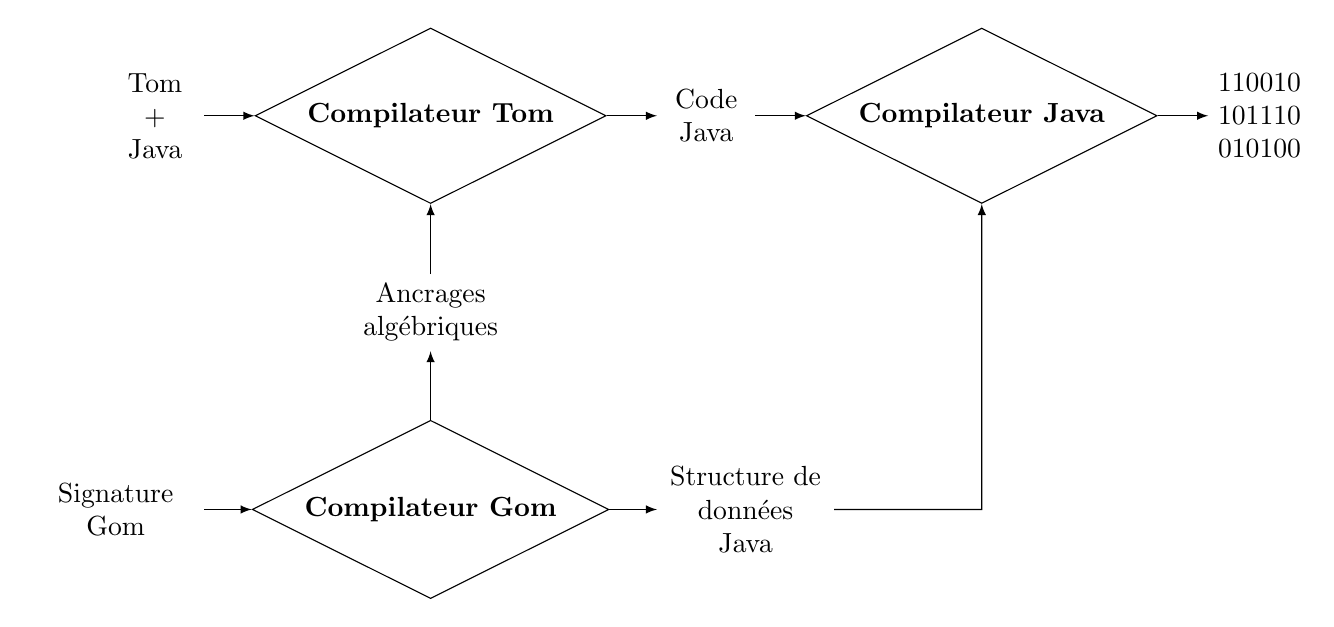
\begin{tikzpicture}[>=latex, node distance=3cm, on grid, auto]
       
       \node[text width=1cm, align=center] (Tom_Java) {Tom \\+ \\Java};
       \node [right=.5, right of=Tom_Java, draw, diamond, aspect=2] (Compilo_Tom) {\textbf{Compilateur Tom}};
       \path[->] (Tom_Java) edge (Compilo_Tom);
       \node[right=.5, right of=Compilo_Tom, text width=1cm,
       align=center] (Code_Java) {Code \\Java};
       \path[->] (Compilo_Tom) edge (Code_Java);
       \node [right=.5, right of=Code_Java, draw, diamond, aspect=2]
       (Compilo_Java) {\textbf{Compilateur Java}};
       \path[->] (Code_Java) edge (Compilo_Java);
       \node [right=.5, right of=Compilo_Java, text width=1cm,
       align=center] (binaire) {110010\\101110\\010100};
       \path[->] (Compilo_Java) edge (binaire);
       \node [below=-.5, below of=Compilo_Tom, text width=2cm,
       align=center] (ancrages) {Ancrages \\ algébriques};
       \path[->] (ancrages) edge (Compilo_Tom);
       \node [below=-.5, below of=ancrages, draw, diamond, aspect=2] (Compilo_Gom) {\textbf{Compilateur Gom}};
       \path[->] (Compilo_Gom) edge (ancrages);
       \node [left=1, left of=Compilo_Gom, text width=2cm,
       align=center] (Sign_Gom) {Signature \\ Gom};
       \path[->] (Sign_Gom) edge (Compilo_Gom);
       \node [right=1, right of=Compilo_Gom, text width=2cm,
       align=center] (Struct_Java) {Structure de \\ données Java};
       \path[->] (Compilo_Gom) edge (Struct_Java);
       \node [right of=Struct_Java] (inv) {};
       \draw[->] (Struct_Java) -- ++(3,0) -- (Compilo_Java);
       
       %\node [draw, diamond, aspect=2] {Compilateur Gom};
       %\node [draw, diamond, aspect=2] {Compilateur Tom};
       

     \end{tikzpicture}
}
\vskip1ex
\caption{TomGomCompiler}
    \end{figure}
  \end{center}

\end{frame}

\end{document}
